\documentclass[a4paper,10pt,twocolumn]{article}

\usepackage[font=small]{caption}
\usepackage{graphicx}
\usepackage{fancyhdr}
\usepackage{amsmath}
\usepackage{amsfonts}
\usepackage[utf8]{inputenc}
\usepackage[brazil]{babel}
\usepackage{titlesec}
\usepackage[numbers]{natbib}
\usepackage{float}
\usepackage{multirow}
\usepackage[includehead]{geometry}


% Geometry settings
\geometry{
    % Margins
    a4paper,
    left=2.6cm,
    right=2.6cm,
    top=1.8cm, % 3.3cm - imageheight/2
    bottom=4.2cm,
    % Text
    columnsep=0.8cm,
    headheight=3.15cm, % imageheight + 0.15cm
    headsep=0.6cm     % Adjust the space between the header and the text
    % Column width = 7.5cm is already satisfied
}

% Define the size of the image
\newlength{\imagewidth}
\newlength{\imageheight}
\setlength{\imagewidth}{3cm}
\setlength{\imageheight}{3cm}

% Header image
\pagestyle{fancy}
\fancyhf{}
\fancyhead[L]{
\includegraphics[width=\imagewidth, height=\imageheight]{Figures/logo_33_pt.pdf}} % Set image size to 3x3 cm
\renewcommand{\headrulewidth}{0pt}

% Font settings for Arial and identation
\renewcommand{\rmdefault}{phv}
\renewcommand{\sfdefault}{phv}
\setlength{\parindent}{0pt}
\raggedbottom


% Title and section settings
\titleformat{\section}{\large\bfseries\centering}{\thesection}{1em}{}
\titlespacing*{\section}{0pt}{2pt}{2pt}
\newlength{\titlespace}
\setlength{\titlespace}{0.4cm}

% Caption settings for figures and tables
\captionsetup{font=small,justification=centering}

\begin{document}
\pagenumbering{gobble}

\title{
    \vspace*{-0.8cm}
    {\fontsize{13}{13}\textbf{TÍTULO}}
    \vspace*{-0.1cm}
}
\author{
    \textbf{Estudante(s) de Graduação Autor(es)}
    \vspace*{\titlespace}
    \\
    \textbf{Colaboradores (máximo 3)}
    \vspace*{\titlespace}
    \\
    \textbf{Orientador(a)}
    \vspace*{\titlespace}
    \\
    Faculdade/Universidade
    \vspace*{\titlespace}
    \\
    \normalsize{E-mail do primeiro autor}
}
\date{}
\maketitle

% Ensure logo appears on the first page
\thispagestyle{fancy}

\section*{Objetivos}

Lorem ipsum dolor sit amet, consectetur adipiscing elit. Quisque laoreet porttitor mauris at tincidunt. Aliquam consequat vehicula lacus, in tempor nisi pulvinar mattis. Donec pulvinar purus eu enim scelerisque in suscipit velit pulvinar.

Vestibulum ullamcorper luctus ipsum, vel sollicitudin turpis vestibulum vel. Curabitur quis ligula ut diam ullamcorper rhoncus. Aliquam ac tortor vitae eros tempor rhoncus. Pellentesque scelerisque, metus sed interdum sodales, diam elit rhoncus est, at faucibus lacus erat nec est.

Donec massa metus, ultricies sed molestie ac, sodales vel est. Sed est eros, lobortis vitae semper vel, elementum sit amet felis. Lorem ipsum dolor sit amet, consectetur adipiscing elit. Quisque laoreet porttitor mauris at tincidunt. Aliquam consequat vehicula lacus, in tempor nisi pulvinar mattis.

Donec pulvinar purus eu enim scelerisque in suscipit velit pulvinar. Vestibulum ullamcorper luctus ipsum, vel sollicitudin turpis vestibulum vel. Curabitur quis ligula ut diam ullamcorper rhoncus. Aliquam ac tortor vitae eros tempor rhoncus. Pellentesque scelerisque, metus sed interdum sodales, diam elit rhoncus est, at faucibus lacus erat nec est.

\section*{Métodos e Procedimentos}

Integer dui nisi, dapibus vitae posuere id, viverra in lorem. Proin dignissim tempor eros, a aliquam orci convallis vitae. Morbi et lectus turpis, vel mattis turpis. Morbi dui dui, consequat sed egestas non, sagittis sed ligula. Etiam sed metus velit. Praesent ac erat metus. Fusce aliquam luctus mauris, vel tempus tortor mollis at. Etiam dictum gravida velit at sagittis. Proin vel augue sit amet velit luctus rutrum vitae id elit. Nullam vel adipiscing felis. Sed condimentum blandit vulputate.

Integer dui nisi, dapibus vitae posuere id, viverra in lorem. Proin dignissim tempor eros, a aliquam orci convallis vitae. Morbi et lectus turpis, vel mattis turpis. Morbi dui dui, consequat sed egestas non, sagittis sed ligula. Etiam sed metus velit. Praesent ac erat metus. Fusce aliquam luctus mauris, vel tempus tortor mollis at. Etiam dictum gravida velit at sagittis. Proin vel augue sit amet velit luctus rutrum vitae id elit. Nullam vel adipiscing felis. Sed condimentum blandit vulputate.Etiam dictum gravida velit at sagittis. Proin vel augue sit amet velit luctus rutrum vitae id elit.

A equação \eqref{eq: langevin for the phase} é uma equação exemplo.

\begin{equation}
    \Delta \Phi(t) =-\gamma \int_{0}^{t} \dot{\mathbf{r}}\left(t_{1}\right) \int_{0}^{t_{1}} \mathbf{G}\left(t^{\prime}\right) d t^{\prime} d t_{1}.
    \label{eq: langevin for the phase}
\end{equation}

Proin dignissim tempor eros, a aliquam orci convallis vitae. Morbi et lectus turpis, vel mattis turpis. Morbi dui dui, consequat sed egestas non, sagittis sed ligula. Etiam sed metus velit. Praesent ac erat metus. Fusce aliquam luctus mauris, vel tempus tortor mollis at. Etiam dictum gravida velit at sagittis. Proin vel augue sit amet velit luctus rutrum vitae id elit. Nullam vel adipiscing felis. Sed condimentum blandit vulputate.

\section*{Resultados}

Curabitur molestie fermentum massa ac sollicitudin. Sed sagittis, dolor eget molestie gravida, lorem diam blandit nunc, ut consequat ipsum metus vel dolor. Nulla vestibulum commodo convallis. Ut tincidunt leo nec risus tristique dignissim. Duis a nisi posuere magna mollis tincidunt non at sapien. Class aptent taciti sociosqu ad litora torquent per conubia nostra, per inceptos himenaeos.

A Figura \ref*{fig:sample_figure} é uma figura exemplo.

\begin{figure}[htbp]
    \centering
    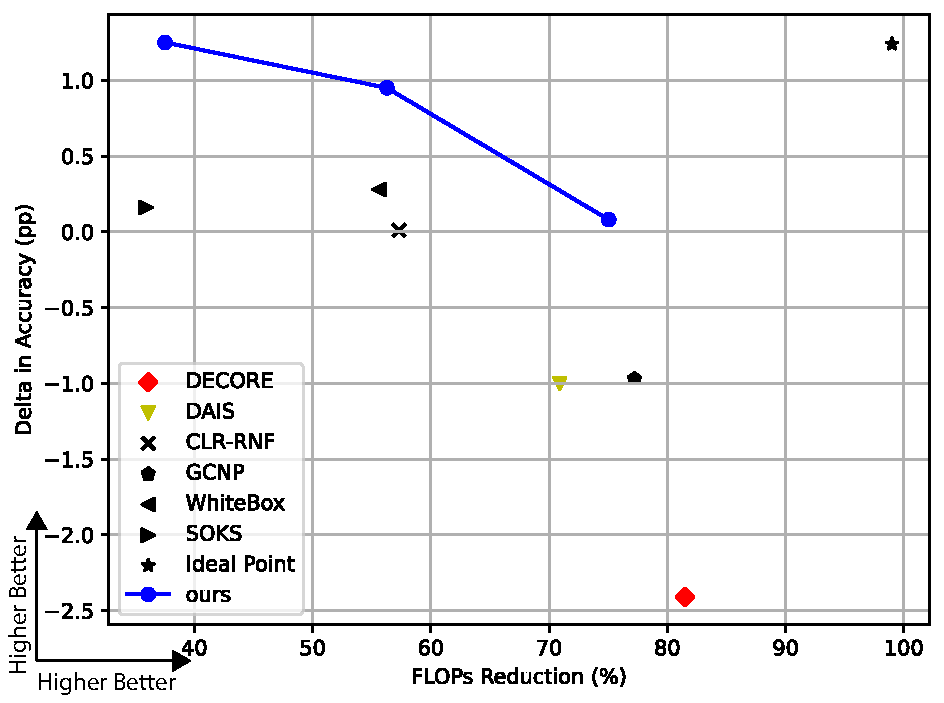
\includegraphics[width=\linewidth]{Figures/sample_figure.pdf}
    \caption{Figura de exemplo.}
    \label{fig:sample_figure}
\end{figure}

\section*{Conclusões}

Nulla facilisi. Mauris luctus elit at urna dignissim eu dictum ante tincidunt. Morbi eros justo, sollicitudin eget aliquam vitae, ultrices et nibh. Nulla nec sapien eu turpis aliquet consectetur at a dolor. Vivamus non dui justo. Etiam leo velit, auctor in faucibus nec, tincidunt sit amet mauris. Integer dignissim hendrerit orci.

Nulla facilisi. Mauris luctus elit at urna dignissim eu dictum ante tincidunt. Morbi eros justo, sollicitudin eget aliquam vitae, ultrices et nibh. Nulla nec sapien eu turpis aliquet consectetur at a dolor. Vivamus non dui justo. Etiam leo velit, auctor in faucibus nec, tincidunt sit amet mauris. Integer dignissim hendrerit orci.

Essa é uma citação exemplo~\cite{example1, example2}.

Nulla facilisi. Mauris luctus elit at urna dignissim eu dictum ante tincidunt. Morbi eros justo, sollicitudin eget aliquam vitae, ultrices et nibh. Nulla nec sapien eu turpis aliquet consectetur at a dolor. Vivamus non dui justo. Etiam leo velit, auctor in faucibus nec, tincidunt sit amet mauris. Integer dignissim hendrerit orci.

A Tabela \ref*{tab:results} é um exemplo de tabela.

\begin{table}[t]
    \centering
    \renewcommand{\arraystretch}{1.2}
    \caption{Tabela de exemplo.}
    \resizebox{\columnwidth}{!}{ % Scale table to fit the single column width
    \begin{tabular}{cccc}
    \hline
    Base de Dados & Modelo & Acurácia (\%) & Tempo (s) \\ \hline
    \multirow{6}{*}{Facies} 
    & XGBoost   & 90.40                & 0.272                        \\
    & XGBoost*  & 91.50                & 4.754                        \\
    & LightGBM  & 90.20                & 0.277                        \\
    & LightGBM* & 90.70                & 0.277                        \\
    & CatBoost  & 89.30                & 3.095                        \\
    & CatBoost* & 91.10                & 3.075                        \\ \hline
    \multirow{7}{*}{MHAD}   
    & XGBoost   & 85.60                & 1.012                        \\
    & XGBoost*  & 87.30                & 5.892                        \\
    & LightGBM  & 84.70                & 0.998                        \\
    & LightGBM* & 86.50                & 1.017                        \\
    & CatBoost  & 83.40                & 2.567                        \\
    & CatBoost* & 85.80                & 2.432                        \\
    & TabPFN    & 88.10                & 3.224                        \\ \hline
    \end{tabular}}
    \label{tab:results}
\end{table}
\textbf{Inserir ao final das conclusões a declaração de conflito de interesses e a contribuição de cada autor (exemplos abaixo):}

Os autores declaram não haver conflito de interesses.\\
OU\\
Os autores declaram os seguintes conflitos de interesse: [descrever brevemente].\\
Autor A concebeu e planejou o estudo. Autor B realizou a coleta e análise dos dados. Autor C participou da redação e revisão final do manuscrito. Todos os autores aprovaram a versão final do resumo.

\section*{Agradecimentos (opcional)}

Lorem ipsum dolor sit amet, consectetur adipiscing elit. Quisque laoreet porttitor mauris at tincidunt. Aliquam consequat vehicula lacus, in tempor nisi pulvinar mattis. Donec pulvinar purus eu enim scelerisque in suscipit velit pulvinar.

\bibliographystyle{ieeetran[pt-br]}
\bibliography{references} % This points to the references.bib file

\end{document}
